\chapter{LBM在GPU上实现的基本方法}
本章介绍了目前文献中常见的LBM在GPU上的实现方法,着重讨论了影响程序性能的因素,并指出了其基本优化策略。
随后我们分别编制了模拟顶盖驱动二维方腔流和外力驱动三维方截面直管道流的GPU程序,在验证了程序正确性后
我们对其运行速度做了测试和分析。

\section{LBM在GPU上实现的基本方法}\label{optimize}
%LBM计算时间主要消耗在碰撞、迁移和统计宏观量等过程,所以只需将这些过程在GPU上实现。
由于GPU和CPU的构架存在巨大差异,很多适用于CPU的优化技术在GPU上可能根本就行不通,甚至
适得其反。例如CPU的LB程序中通常要避免数组的第一个维度大小为2的幂次,这是考虑到CPU缓存效率
的缘故\ucite{wellein2006single},而在GPU上情况却恰恰相反。下面将从LBM算法的特点结合GPU构架
特点来分析在GPU上实现高效LBM计算应该采取的策略。

在LBM计算过程中,每个格点
速度分布函数方向很多,但其碰撞步执行的计算却很简单,在迁移步甚至没有计算而只是简单的数据
加载与存储,因此LBM的计算访存比较大,在已经充分优化的情况下,程序的性能瓶颈还是在访存带宽,
并且在CPU上和GPU上都是如此\ucite{tolke2010implementation}。考虑到这一特点,LBM在GPU上的实现
及优化目标为最大限度发挥GPU的带宽优势,即尽量提高访存效率。下面将从数据布局和存储器使用方面
介绍LBM在GPU上实现的关键之处。

\subsection{优化数据布局}
%为了实现全局存储器的连续访问
在CPU上实现LBM时,速度分布函数(PDF)在内存中有两种最为常见的布局方式\---结构数组
(Arrays of Structure, AoS)和数组结构(Structure of Arrays,SoA)\ucite{wellein2006single}。
前者是指每个格点的$q$个PDF在内存中是连续排布的,而后者是指不同格点同一方向的PDF在
内存中是连续排布的。如果用C语言的数组记法表示,对于前者分布函数声明为\verb+f[NZ][NY][NX][Q]+,
而对于后者则为\verb+f[Q][NZ][NY][NX]+。在GPU实现时,为了保证相邻线程在同一时刻访问全局内存的
地址是连续的,只能采用后一种形式,即SoA。

\subsection{减少全局内存访问}
LBM计算在逻辑上可以分为三个步骤即碰撞、迁移、更新宏观量,如果分开执行这些操作,
则会多次从全局内存加载和存储数据。事实上利用LBM是一种显式方法这个特点,这三个逻辑
步骤可以合并在一个Kernel中执行。
通常在全局内存上开辟有两套PDF数组,如\verb+F0+和\verb+F1+,在一个时间步,每个格点
从\verb+F0+中加载自己的PDF,随后计算宏观量,然后执行碰撞,并将新的PDF写入到
\verb+F1+中相邻格点对应的位置,在下一时间步执行相同操作,不过读取和写入位置置换,
即从\verb+F1+中读取,碰撞后写入\verb+F0+。
注意在上述方法中迁移步已经掩藏在向周围点写入新PDF的过程中了。

\subsection{利用共享内存辅助迁移过程}\label{sec:cuda_share}
在迁移过程中每个格点不可避免地要从临近格点写入PDF,如果临近格点的$X$坐标(这里假定
按\verb+f[Q][NZ][NY][NX]+形式开辟数组)与自己不同,则写入过程肯定有一个\verb+sizeof(type)+
的偏移,因而不能不满足内存对齐要求,实际显存带宽会大为下降。目前常见的做法是用共享内存
辅助迁移。即格点首先将自己的PDF读到自己的共享内存中,完成碰撞操作后从共享内存将数据写
回全局内存,穿出Block边界的PDF正好可以临时存在Block另一侧空出的位置,
图\ref{fig:share_shift}所示为向右迁移的情况。
写会过程中从共享内存读的是相邻格点的数据,而写入全局内存时的是写到自己的位置。
总体上看,读写全局内存时都满足内存地址对齐要求,理论存储效率可以达到100\%。
\begin{figure}[htb]
  \centering
  \begin{tikzpicture}
    \matrix (block) [matrix of nodes, row sep=2.0em ,nodes={draw,  minimum width=2em, anchor=center} ]
    {
      0 & 1 & 2 & 3 \\
      0 & 1 & 2 & 3 \\
      0 & 1 & 2 & 3 \\
    };

    \draw (block-1-1.west) + (-1.0, 0) node {\hei \small 全局内存};
    \draw (block-2-1.west) + (-1.0, 0) node {\hei \small 共享内存};
    \draw (block-3-1.west) + (-1.0, 0) node {\hei \small 全局内存};

    \draw[->,thick] (block-1-1.south) -- (block-2-1.north);
    \draw[->,thick] (block-1-2.south) -- (block-2-2.north);
    \draw[->,thick] (block-1-3.south) -- (block-2-3.north);
    \draw[->,thick] (block-1-4.south) -- (block-2-4.north);

    \draw[->,thick] (block-2-1.south) -- (block-3-2.north);
    \draw[->,thick] (block-2-2.south) -- (block-3-3.north);
    \draw[->,thick] (block-2-3.south) -- (block-3-4.north);
    \draw[->,thick] (block-2-4.south) -- (block-3-1.north);
  \end{tikzpicture}
  \caption{利用共享内存辅助迁移}
  \label{fig:share_shift}
\end{figure}

\begin{figure}[htpb]
  \centering
  \includegraphics[]{img/exchange}
  \caption{\textbf{LBExchange}执行过程}
  \label{fig:lbexchange}
\end{figure}

由于在迁移过程中穿越Block边界的PDF没有被存到显存中正确的位置,所以在执行完碰撞步的Kernel
后还要紧跟着调用另外一个Kernel来完成迁移步,这里我们按原文献命名为\textbf{LBExchange}。
它的作用就是交换这些没有被迁移到正确位置的PDF。在三维情况,由于存储空间限制,不可能
所有方向网格数都很大,如不会都超过$128$或$256$,这时正好可以让一个相应大小的一维Block
处理网格数最小的方向上的“一条”格点,
这时可以不用执行\textbf{LBExchange} Kernel,而只需做一般的边界处理。
\ref{sq}节中的方截面直管道流动模拟
就利用了这个特点。

\section{验证算例及性能测试} \label{sec:speed_standard}
这一节简要列出利用上节所述方法实现的不同算例GPU程序的程序性能,并将计算结果与相关文献或解析解做了对比
以验证程序的正确性。
\subsection{计算环境及程序性能测量方法}
本工作使用的计算环境一台服务器搭载Tesla C1060型GPU的服务器,GPU标配显存4GB,
CPU为Intel Xeon X5550 8核处理器,操作系统为CentOS 5.9 64bit版,CUDA工具箱版本为3.2。
%使用Intel 的icc编译器,版本号为12.0.2。
%PC机搭载GeForce系列GTX480 GPU,CUDA工具箱版本为5.0,CPU为 AMD Athlon II X4 640。
本文中所有CPU程序均为串行程序,使用icc V10.1编译器编译,编译选项加上了\verb+-fast+。

衡量LBM程序速度的标准单位是MLUPS(Million Lattice Updates Per-second),
意为每秒百万节点更新数。按照这个单位,程序运行速度其定义为
\begin{equation}
  \text{Speed} = \frac{N_{\text{total}}\times T_{\text{LB}}}{10^6\times t_{\text{comput}}} \text{(MLUPS)}
  \label{mlups}
\end{equation}
其中$N_{\text{total}}$表示流场中格点总数,$T_{\text{LB}}$表示总的LB演化步数,
$t_{\text{comput}}$表示计算$T_{\text{LB}}$步所消耗的时间。
考虑多孔介质流动情况时,还有一个只考虑流体格点的衡量单位\---
MFLUPS,其定义与MLUPS相比只是分子的$N_{\text{total}}$换为流体格点总数。
因为多孔介质中存在大量不参与计算的固体格点,所以这个单位才能真实反映计算速度。

这里我们指出在计算GPU程序相对于CPU程序加速比时,CPU程序性能对加速比影响很大(作为分母),
而实际CPU程序执行的速度在相当程度上取决于CPU性能和所使用的编译器及编译选项,所以笼统的
指出GPU程序的加速比并能不准确放映GPU程序的加速效果。在后文的性能测试中我们主要
以MLUPS和MFLUPS为单位衡量GPU程序的绝对速度。

\subsection{二维方腔流}
二维方腔流边界条件简单,但是随雷诺数增大,却可以产生复杂的涡结构,因此被广泛地
用作验证程序正确性的标准算例\ucite{ghia1982high}。
这里我们采用的方腔流几何结构如图\ref{fig:ldc_a}所示,方腔四边长都为1.0m,空腔上边界以恒定速度$U=0.1\text{m/s}$水平向右移动。
我们对比了雷诺数为400时的GPU程序计算结果与Ghia\ucite{ghia1982high}等人的用多重网格方法计算得出的结果,
并将GPU程序和对应的CPU程序计算速度作了对比。

我们采用的是标准D2Q9 LBGK模型,固壁采用半反弹格式,上边界采用非平衡外推格式,网格数为$256\times 256$,
在GPU上采用单精度计算,收敛标准为
\begin{equation}
  \frac{\sqrt {\sum\nolimits_{ij}{| \bm u_{ij}^{n+1000}- \bm u_{ij}^{n} |^2}}}{\sqrt{\sum\nolimits_{ij}{|  \bm u_{ij}^{n} |^2}}}\le 1.0\times {{10}^{-6}}
  \label{convege}
\end{equation}
表示相邻1000步直间速度场的相对误差小于$1.0\times 10^{-6}$。 
图\ref{fig:ldc_b}所示为流场稳定后的流线图,可以发现有三个涡结构分别出现在方腔中心和左、右下角。表
\ref{tab:ldc}列出了本文计算出的涡中心位置以及Ghia\ucite{ghia1982high}的结果,可以看出本文结果和Ghia
的结果相差很小。
\begin{figure}[htb]
  \centering
  \subfigure[二维方腔流示意图]{
    \begin{minipage}[b]{0.4\textwidth}
      \includegraphics[width=1\textwidth]{img/ldc}
      \label{fig:ldc_a}
    \end{minipage}
  }
  \subfigure[$Re=400$时稳定后流线图]{
    \begin{minipage}[b]{0.38\textwidth}
      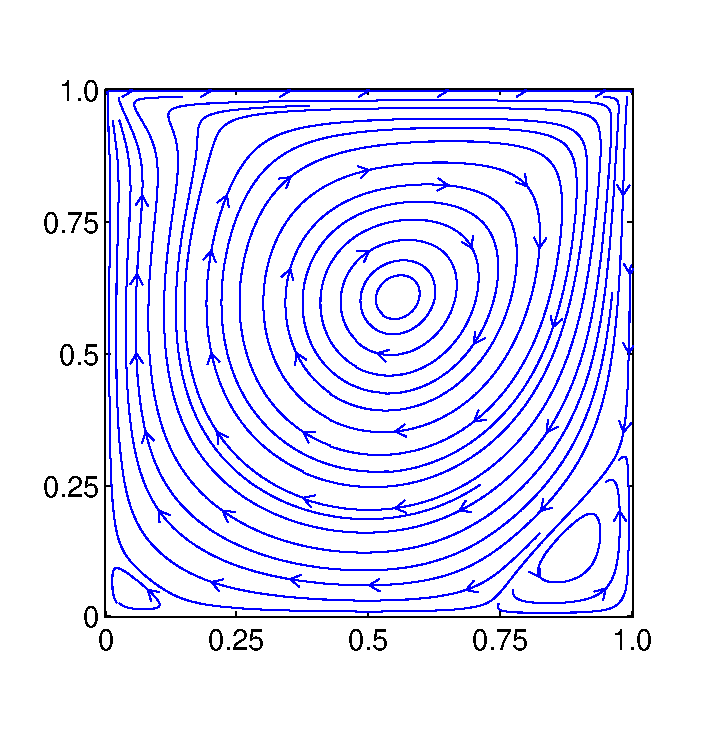
\includegraphics[width=1\textwidth]{img/ldc_stream}
      \label{fig:ldc_b}
    \end{minipage}
  }
  \caption{二维方腔流}
\end{figure}

\begin{table}
  \centering
  \begin{tabular}{*{7}{c}}
    \toprule
涡    & \multicolumn{2}{c}{一级涡} & \multicolumn{2}{c}{二级涡} & \multicolumn{2}{c}{三级涡}  \\ \cline{2-3} \cline{4-5} \cline{6-7}
位置    & $x_1$ & $y_1$              & $x_2$ & $y_2$              & $x_3$ & $y_3$          \\ \midrule
本文& $0.5543$ & $0.6070$        & $0.8889$ & $0.1235$        & $0.0522$ & $0.0475$        \\ \hline
Ghia& $0.5547$ & $0.6055$        & $0.8906$ & $0.1250$        & $0.0508$ & $0.0469$        \\ \bottomrule
  \end{tabular}
  \caption{$Re=400$时,各级涡中心的位置}
  \label{tab:ldc}
\end{table}

我们发现Block的大小(本文采用的Block是一维的)和总体网格规模对计算速度都有影响,图\ref{fig:ldc_speed}所示为
不同Block大小和不同网格规模时的计算速度,可以发现GPU最快速度快达到924MLUPS,而与之相比,我们的CPU
程序速度为7.5MLUPS,可见GPU程序加速比达到了123倍。

\begin{figure}[htb]
  \centering
  %\psfig{figure=img/ldc_speed}
  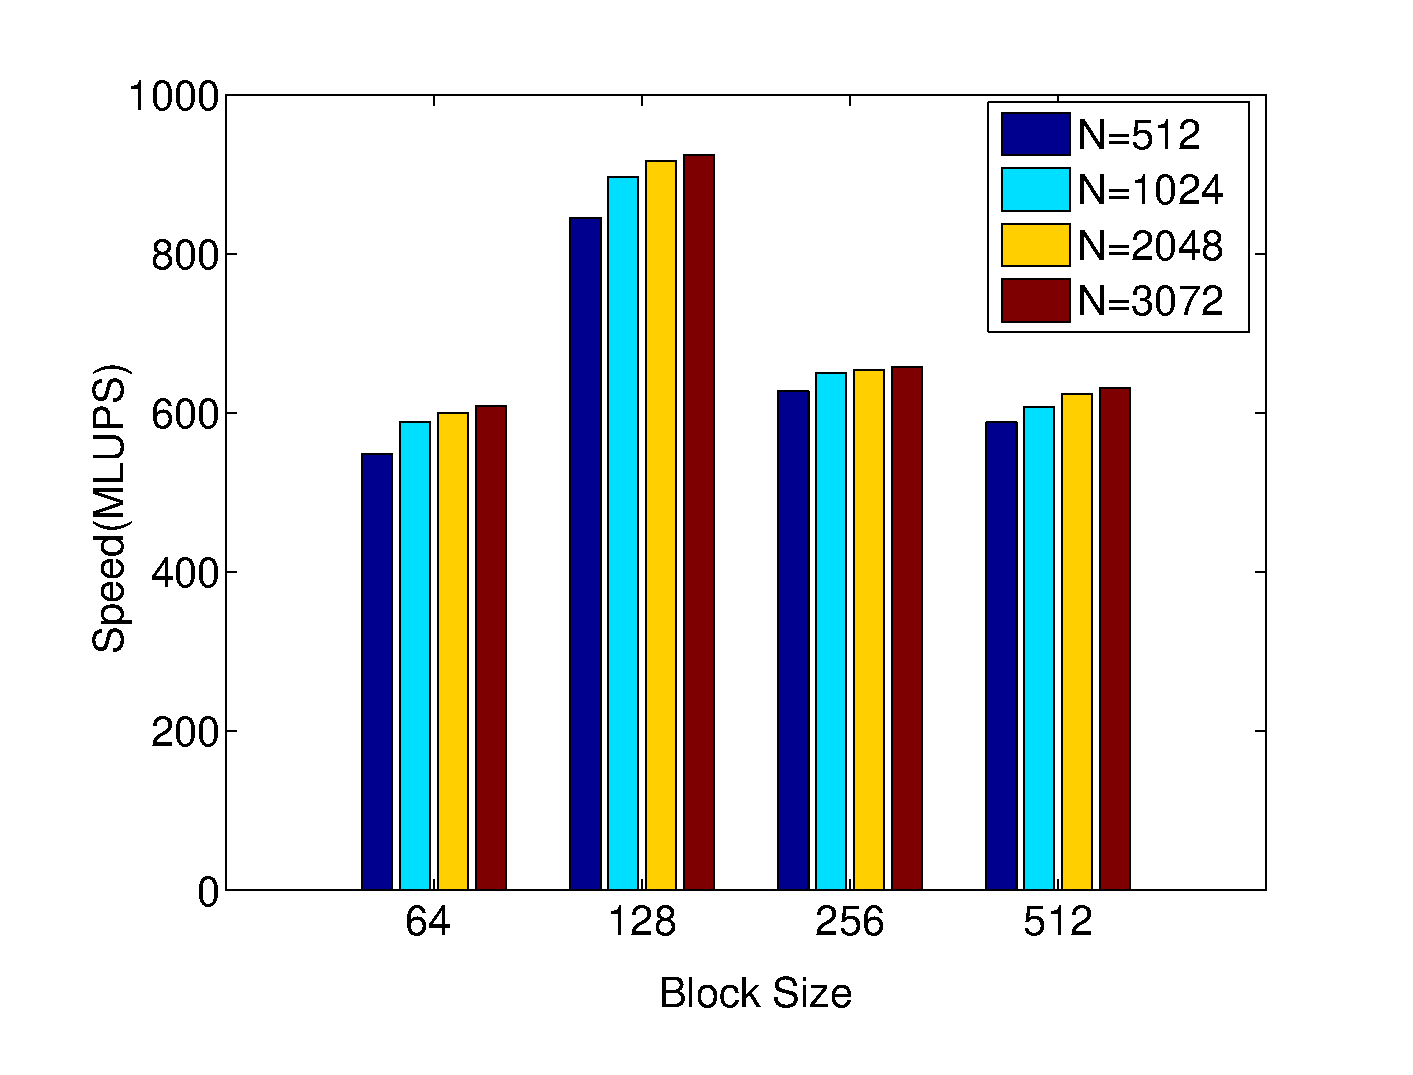
\includegraphics[width=0.8\textwidth]{img/ldc_speed}
  \caption{网格规模和不同Block尺寸对计算速度的影响}
  \label{fig:ldc_speed}
\end{figure}

\subsection{方形截面直管道流动}\label{sq}
本小节将依然使用\ref{optimize}节中描述的方法模拟三维方形截面直管道流动,
如图\ref{fig:sq}所示,这种流动类似于二维的
泊肃叶流动,流体由沿管道方向的外力$\bm F$驱动。
由于流动沿管道方向具有周期性,所以管道长度不影响截面速度分布。
截面流向速度分布只取决于外力大小$\bm F$和管道宽度$a$,其级数解析解为
\begin{equation}
  u(x, y) = U_0\sum_{i=1}^{\infty}(-1)^i\left(1-\frac{\cosh(\pi xi/a)}{\cosh(\pi i/2)}\right)\frac{\pi yi/a}{i^3}
  \label{sq_ana}
\end{equation}
其中$U_0=\frac{4aF}{\nu \pi^3}$。

\begin{figure}[htb]
  \centering
  \subfigure[几何结构]{
    \begin{minipage}[b]{0.6\textwidth}
      \includegraphics[width=0.9\textwidth]{img/sqpng}
      \label{fig:sq}
    \end{minipage}
  }
  \subfigure[管道截面示意图]{
    \begin{minipage}[b]{0.2\textwidth}
      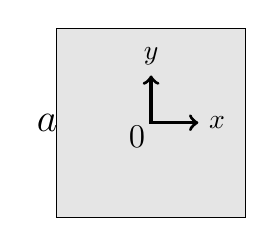
\begin{tikzpicture}[scale=0.6]
        \draw[fill=gray!20]  (-2,-2) rectangle (2,2);
        \draw [<->,very thick] (0,1) node (yaxis) [above] {$y$} |- (1,0) node (xaxis) [right] {$x$};
        \node at (-2.2, 0) {\Large $a$};
        \node at (-0.3, -0.3) {\large $0$};
      \end{tikzpicture}
      \label{fig:sq_sec}
    \end{minipage}
  }
  \caption{外力驱动方截面直管道流}
\end{figure}
数值模拟采用D3Q15标准LBGK模型,管壁边界采用非平衡态外推格式处理。参数$U_0=0.001$, 收敛标准仍热使用式\eqref{convege}。
计算收敛后与解析解的相对误差为$0.14\%$。
其中$y=0$处速度分布与解析解的对比见图\ref{fig:sq_vx}。
%\begin{figure}[htb]
%  \centering
%  %\subfigure[截面速度分布]{
%    %\begin{minipage}[b]{0.6\textwidth}
%  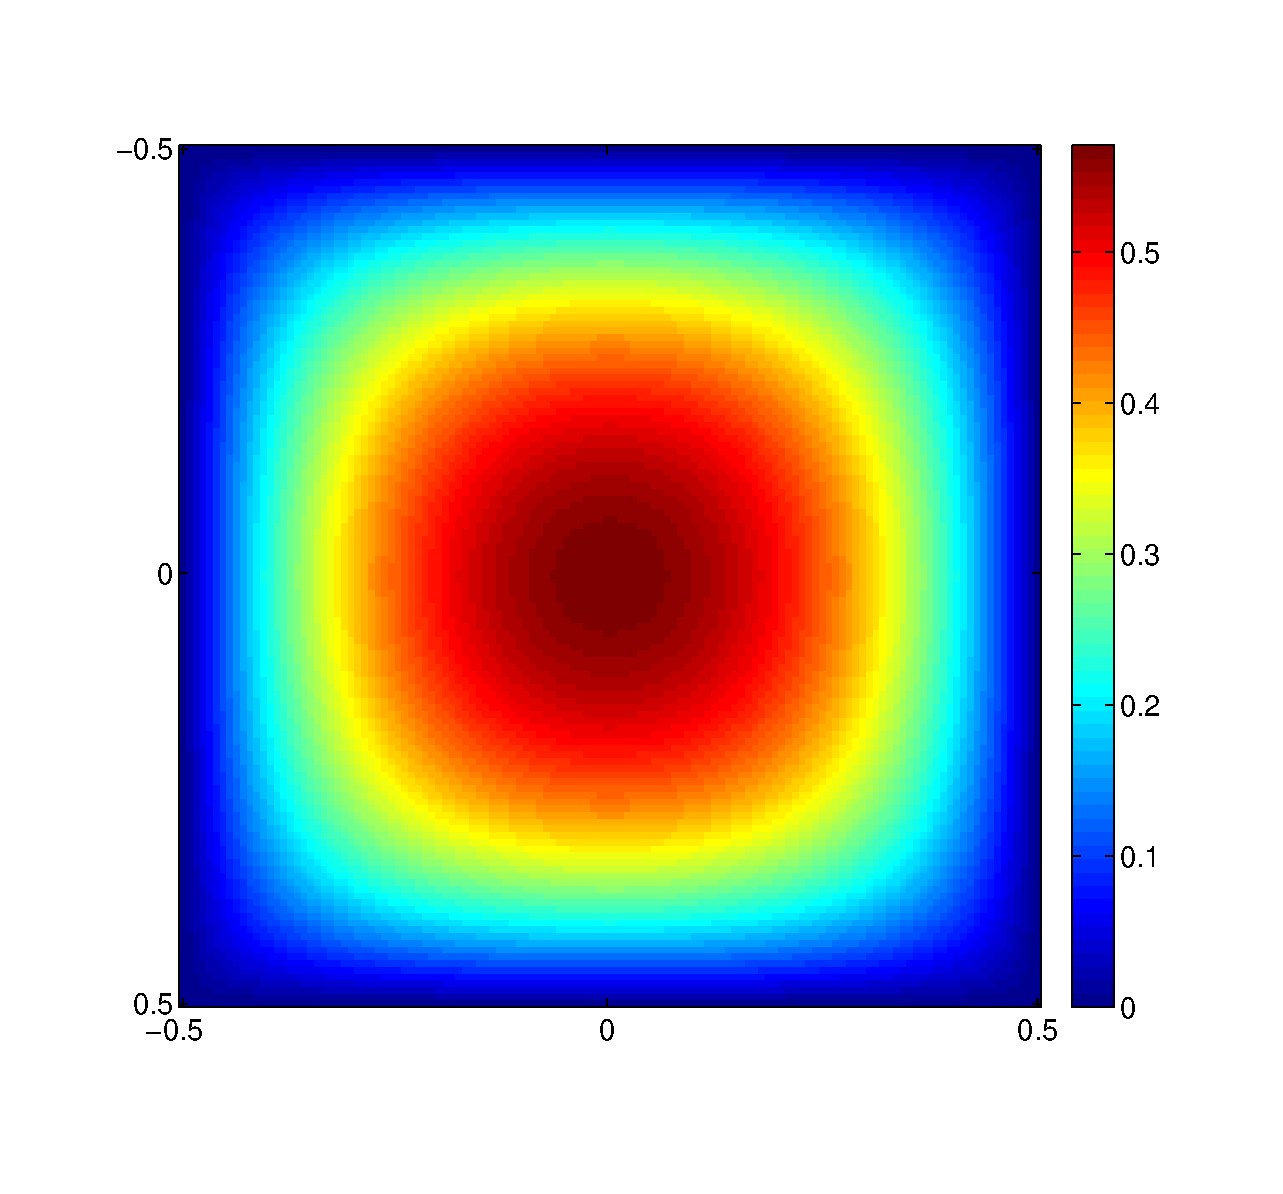
\includegraphics[width=0.6\textwidth]{img/sq_vx}
%  \label{fig:sq_vx}
%  \caption{截面速度}
%\end{figure}
    %\end{minipage}
  %}
  %\\
  %\subfigure[$y=0$处速度分布]{
    %\begin{minipage}[b]{0.6\textwidth}
\begin{figure}[htb]
  \centering
  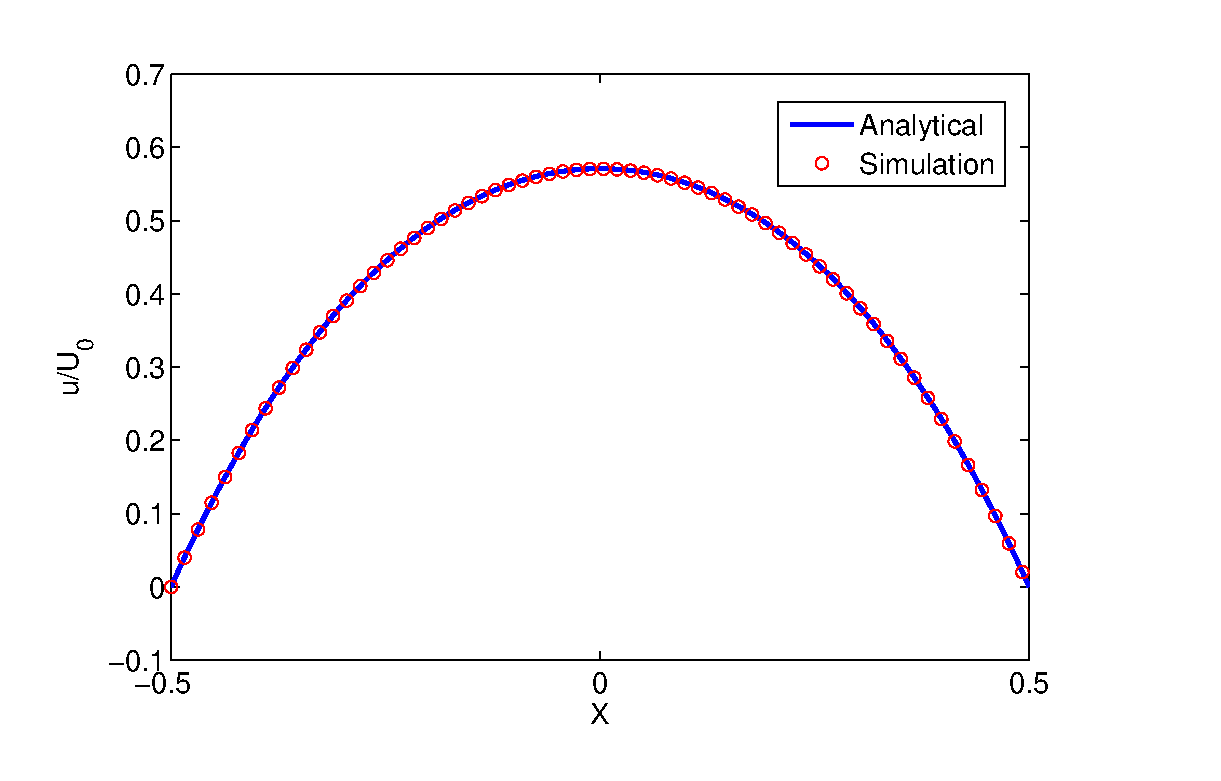
\includegraphics[width=0.7\textwidth]{img/sq_u}
  \caption{截面上$y=0$处速度与解析解比较}
   \label{fig:sq_vx}
    %\end{minipage}
  %}
\end{figure}
%\subsection{圆柱绕流}
%\subsection{简单二维多空介质流动}
GPU程序中由于采用了4.1节中指出的方法,可以不用另外执行\textbf{LBExchange} Kernel,
因为流出Block的PDF又流回到了Block的另一侧,这正好符合周期性边界实现方式。
固壁边界需要另外的Kernel来进行非平衡外推处理。 我们对不同Block尺寸和不同网格规模
下的计算速度做了测试,结果如图\ref{fig:sq_speed}所示。作为对比,CPU程序在不同网格规模
下的计算均为$4\sim5$MLUPS左右。可见我们实现的GPU程序最快可以加速两个量级以上。
\begin{figure}[htb]
  \centering
  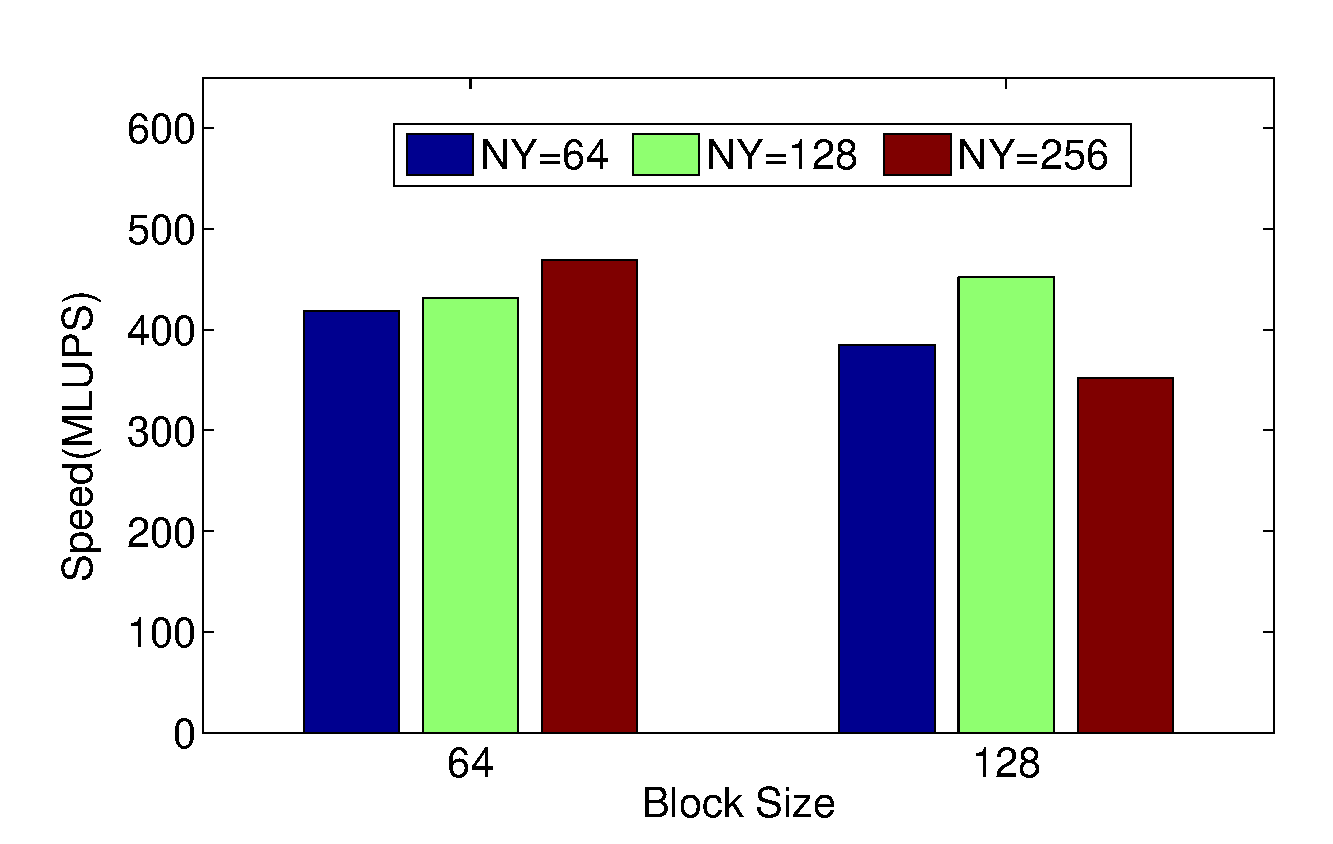
\includegraphics[width=0.6\textwidth]{img/sq_speed}
  \caption{不同Block尺寸和网格规模下的计算速度}
  \label{fig:sq_speed}
\end{figure}

\section{小结}
本章首先介绍了LBM在GPU上实现的基本方法及优化策略,然后利用按照这些方法
实现的GPU程序模拟了二维方腔流和三维方形截面直管道流。模拟结果均与解析解
或参考文献吻合良好,证明GPU程序正确的实现了LBM算法。
之后又测试了GPU程序性能,并考察了影响计算速度的因素。两个算例的GPU程序
的计算速度均为CPU版本的两个量级以上。下一章,我们将考虑流固边界较为复杂的
渗流问题。

